\chapter{Mở đầu}
\label{chap:introduction}

Từ xưa tới nay, giao vận luôn là một trong những ngành đóng vai trò quan trọng trong nền kinh tế. Giao vận và quản lý chuỗi cung ứng đóng vai trò là một cầu nối giữa các đơn vị sản xuất và người tiêu dùng. Nó cũng là một trong những ngành có ảnh hưởng lớn đến sự phát triển của một quốc gia. 

Từ những thập niên 90 của thế kỉ trước, thời kì bùng nổ của Internet đã thúc đẩy một hình thức bán hàng hoàn toàn mới, đó là bán hàng trực tuyến. Hàng loạt các sàn thương mại điện tử lớn ra đời, có thể kể đến như Amazon (Mỹ - 1994), Alibaba (Trung Quốc - 1999), Rakuten (Nhật Bản - 1997). Ngày nay các sàn thương mại điện tử này trở thành những công ty hàng đầu thế giới không chỉ ở lĩnh vực bán hàng mà là cả công nghệ. Việc phát triển vũ bão của các sàn thương mại điện tử dẫn đến số lượng hàng hóa được tiêu thụ trên toàn cầu tăng lên một cách đáng kinh ngạc so với bán hàng truyền thống. Logistic và quản lý chuỗi cung ứng là một trong những xương sống của thương mại điện tử cùng với \textit{nền tảng công nghệ}, \textit{nền tảng thanh toán} hay \textit{chăm sóc khách hàng}... Để quản lý, giao vận số lượng đơn hàng lớn như vậy tới tay khách hàng, cách thức làm việc trong ngành logistic cũng phải thay đổi rất nhiều, áp dụng những công nghệ hiện đại hơn cách làm truyền thống.

Một trong những bài toán quan trọng nhất của logistic là bài toán vận tải hay định tuyến xe (hay người giao hàng). Với lượng xe có tải trọng hữu hạn, chúng ta cần định tuyến các xe này để giao hàng cho khách hàng ở các địa điểm khác nhau từ kho. Mục tiêu là tối ưu tổng quãng đường di chuyển của tất cả các xe để giảm chi phí vận hành. Lớp bài toán như vậy được gọi là \textit{Vehicle Routing Problem - VRP}. Phiên bản đơn giản của VRP là TSP (\textit{Travelling Salesman Problem}) hay bài toán người đưa hàng. Trong TSP, chúng ta có một người đưa hàng cần đi qua tất cả các địa điểm để giao hàng và quay trở về điểm xuất phát. TSP hay VRP là nhóm bài toán NP-hard, hiện tại người ta vẫn chưa tìm được lời giải trong thời gian đa thức. Tuy nhiên, với sự phát triển của các thuật toán hiện đại, chúng ta có thể tìm được nghiệm "gần" tối ưu cho nhiều bài toán NP-hard (có kích thước lớn) với chất lượng tương đối cao trong thời gian hợp lý.

VRP lần đầu tiên được giới thiệu bởi Dantzig, George B và Ramser, John H (1959) \cite{dantzig1959truck}, rất sớm trước thời kì bùng nổ Internet những năm 90! Tuy nhiên, cho tới nay, VRP vẫn thu hút được sự quan tâm lớn từ cộng đồng những nhà toán học hay khoa học máy tính bởi tính ứng dụng cao của nó. Với nhu cầu giao vận cùng lượng khách hàng cần phục vụ ngày càng tăng của các doanh nghiệp, việc tối ưu hóa chi phí vận hành là một vấn đề cấp thiết. Nhiều doanh nghiệp đã ứng dụng việc định tuyến tự động thay vì để tài xế tự tìm đường thủ công khi giao hàng như trước kia, thế nên việc tìm ra các tuyến đường "gần" tối ưu cần diễn ra nhanh chóng để tránh người giao hàng, hay lái xe phải chờ lâu để có được lộ trình cần thiết trước khi thực hiện giao hàng. 

Trong luận văn này, tác giả nghiên cứu mô hình toán học của VRP cùng các biến thể của nó và các thuật toán giải quyết bài toán này. Tác giả sử dụng thuật toán ALNS (\textit{Adaptive Large Neighborhood Search - Ropke, Stefan và Pisinger, David (2006)} \cite{ropke2006adaptive}). ALNS được phát triển dựa trên LNS - \textit{Large Neighbourhood Search - Shaw (1997)} \cite{shaw1997new}. Hiệu năng và chất lượng nghiệm của ALNS được đánh giá trên các tập dữ liệu thực tế với số lượng yêu cầu (khách hàng) từ nhỏ tới rất lớn. Tác giả đề xuất một thuật toán hủy mới cho ALNS gọi là \textit{Xóa tuyến tệ} (\textit{Bad Route Removal}) giúp giảm số xe sử dụng một cách nhanh chóng. Thêm vào đó, tác giả cũng đề xuất một hiệu chỉnh cho việc tự động điều chỉnh trọng số lựa chọn thuật toán trong ALNS giúp tăng hiệu năng và tiết kiệm tài nguyên so với ALNS gốc một cách đáng kể, thuật toán được đặt tên là B-ALNS (\textit{Boosted - Adaptive Large Neighborhood Search}). Trong thực nghiệm với tập dữ liệu rất lớn với $1000$ yêu cầu, B-ALNS tiết kiệm đến $75\%$ tài nguyên so với ALNS gốc, khi sử dụng cùng một lượng tài nguyên, B-ALNS đạt được kết quả tốt hơn ALNS gốc đến $20\%$ trong thời gian chạy ban đầu của thuật toán.

\begin{figure}[H] % places figure environment here   
  \centering % Centers Graphic
  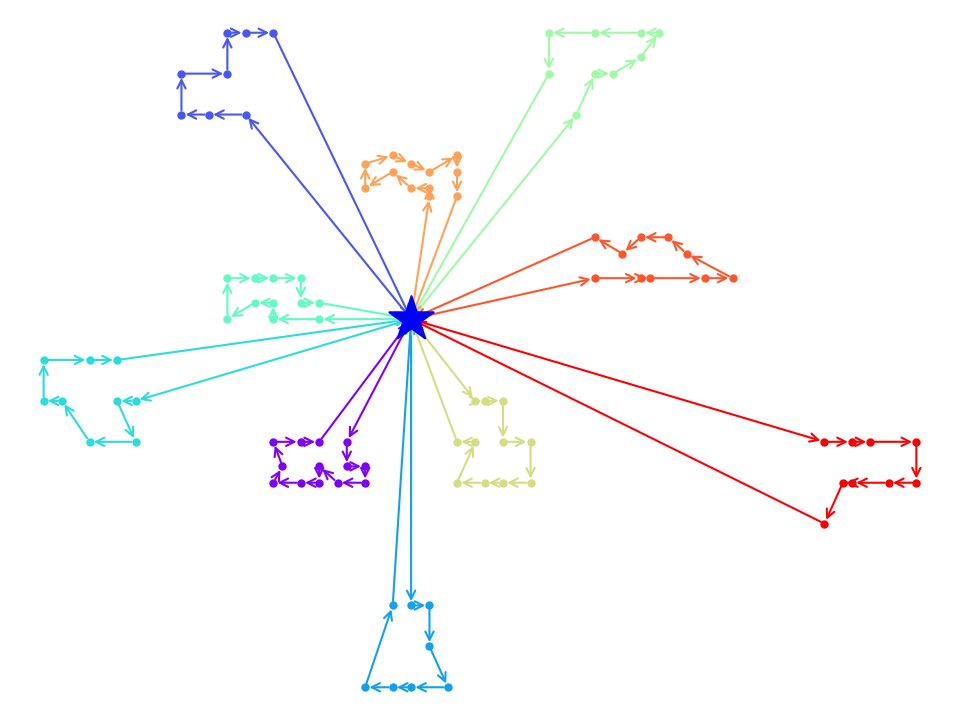
\includegraphics[width=0.9\textwidth]{figures/routes_c101.png} 
  % \includesvg[scale=1]{figures/core-object}
  \caption{VRP với 10 xe phục vụ 100 khách hàng (cấu hình Solomon C101)} 
  % \label{fig:fg_02}
\end{figure}

Các vấn đề được đề cập trong luận văn này được trình bày trong 7 chương. \hyperref[chap:introduction]{Chương 1} giới thiệu vấn đề nghiên cứu \hyperref[chap:model]{Chương 2} phân loại các biến thể của VRP và đưa ra các định nghĩa cũng như mô hình toán học của chúng.
\hyperref[chap:solution]{Chương 3} giới thiệu khái quát một số  phương pháp giải quyết VRP đã được nghiên cứu trước đó.
\hyperref[chap:search]{Chương 4}  trình bày phương pháp tìm kiếm lân cận rộng và thuật toán tìm kiếm lân cận rộng thích ứng.
\hyperref[chap:application]{Chương 5} đưa ra cấu trúc chương trình và các lớp chính được sử dụng để triển khai thuật toán tìm kiếm lân cận rộng thích ứng giải bài toán VRP với ràng buộc khung thời gian.
\hyperref[chap:experiment]{Chương 6} trình bày kết quả thực nghiệm và đánh giá hiệu năng của thuật toán.
\hyperref[chap:conclusion]{Chương 7} tóm tắt lại các kết quả đạt được và đề xuất hướng phát triển trong tương lai.
